\documentclass[10pt]{article}

\usepackage[margin=1in]{geometry}
\usepackage{times}
\usepackage{microtype}
\usepackage{booktabs}
\usepackage{amsmath,amssymb,amsfonts,mathtools}
\usepackage{graphicx}
\usepackage{enumitem}
\usepackage{xcolor}
\usepackage{url}
\usepackage{hyperref}
\usepackage{algorithm}
\usepackage{algpseudocode}
\usepackage{xspace}
\usepackage{multirow}
\usepackage{tikz}
\usepackage{pgfplots}
\pgfplotsset{compat=1.18}
\usetikzlibrary{arrows.meta,positioning,fit,calc,shapes.misc,shapes.geometric}

\hypersetup{colorlinks=true,linkcolor=blue,citecolor=blue,urlcolor=blue}

\newcommand{\method}{\textsc{PACT-V}\xspace}
\newcommand{\methodlong}{Progress-Aware Chunking and Transition Verification\xspace}
\newcommand{\progtok}{\texttt{[PROG]}}
\newcommand{\Hs}{H_s}
\newcommand{\Hl}{H_\ell}
\newcommand{\Sstages}{S}
\newcommand{\Msamples}{M}
\newcommand{\bt}{\tilde{b}_t}
\newcommand{\st}{\tilde{s}_t}
\newcommand{\one}{\mathbf{1}}

\title{\vspace{-0.7em}
\textbf{PACT-V: Progress-Aware Chunking and Transition Verification\\
for Long-Horizon Lightweight Vision-Language-Action Policies}
\vspace{-0.4em}}

\author{Duong Dinh Hieu\\FPT University\\\texttt{email@domain.com}}
\date{}

\begin{document}
\maketitle

\begin{abstract}
Long-horizon robot manipulation is difficult for lightweight
Vision-Language-Action (VLA) policies because small mistakes near subtask
boundaries compound into unrecoverable downstream failures.
This draft focuses on a specific and measurable target failure mode:
\emph{false-positive transitions}, where the controller behaves as if the
current subtask were complete even though the underlying state has not yet
satisfied the corresponding completion predicate.

We present \method\ (\methodlong), a lightweight training-and-inference
recipe that improves \emph{when to replan} and \emph{when to accept a subtask
boundary} without introducing an online planner, a VLM verifier, or a
stage-conditioned policy branch.
The method has three parts.
\textbf{(1) State-grounded boundary supervision:}
ordered subtask predicates from the simulator define persistent completion
boundaries, from which we derive a distinct boundary-imminent label and augment
training with failed rollouts from the frozen base policy.
\textbf{(2) Progress-aware PEFT:}
a learnable \progtok\ token and a lightweight head, trained with LoRA, predict a
stage distribution and a boundary-imminence score from the shared backbone.
\textbf{(3) Verified replanning by prefix execution:}
near suspected boundaries the controller switches from long-prefix execution to
short-prefix execution and evaluates inter-sample variance across multiple
policy action chunks; low variance over consecutive re-observations is treated
as evidence that the current boundary is genuine, while high variance keeps the
controller in short-horizon replanning mode.

This manuscript is intentionally written as a corrected methods paper and
preregistered evaluation protocol.
It removes unsupported empirical claims, fixes the notation and metric issues
in the earlier draft, and makes the scope explicit:
\method\ changes boundary handling and replanning frequency, not the basic VLA
architecture.
We provide a reproducible evaluation plan for SmolVLA on LIBERO-LONG, including
formal definitions of false-positive transition rate, blocked-trigger rate,
boundary recall, and compute overhead.
\end{abstract}

\section{Introduction}

Vision-Language-Action (VLA) models map multimodal observations and natural
language instructions directly to robot actions, offering a scalable route to
general-purpose manipulation~\cite{openvla,rt2,msplora}.
Recent work has shown that smaller and more deployable VLA systems can be built
by reducing visual token counts, reusing pretrained multimodal backbones, and
adapting them with parameter-efficient fine-tuning rather than full retraining~\cite{openvla,msplora}.
SmolVLA is a representative example: a compact open model designed for efficient
training and inference while still using chunked action generation~\cite{msplora}.

What remains hard is \emph{long-horizon composition}.
Benchmarks such as LIBERO include multi-step language-conditioned tasks in which
errors accumulate across sequential manipulation phases~\cite{libero}.
Recent long-horizon VLA work repeatedly highlights failures around subtask
transitions: repeated actions, premature switching, or missed phase changes
cause downstream cascades even when the underlying short-horizon motor skills
are individually adequate~\cite{palm,cyclevla}.

This draft targets one concrete version of that problem:
\textbf{false-positive transition (FPT)}.
An FPT occurs when the controller accepts a subtask boundary before the current
subtask has been completed in the environment state.
Examples include switching from grasp to transport before the object is securely
in hand, or switching from insertion to release before alignment is achieved.
Once such a transition is accepted, later actions are executed from an
out-of-distribution state, and imitation-style policies are well known to suffer
from compounding error under such distribution shift~\cite{ross2011dagger}.

The earlier version of this manuscript had three critical weaknesses.
First, it used the same symbol for both the number of subtasks and the number of
variance samples, which made the algorithm internally inconsistent.
Second, it conflated a boundary-imminent label with a completion label, even
though those represent different events.
Third, it described ``advancing the stage'' during inference even though the
stage index was not actually provided back to the policy, so the claimed
mechanism was stronger than the algorithm being written.

We correct those issues by narrowing the scope and making the method exact.
\method\ is a \emph{boundary-aware replanning controller} built on top of an
existing chunked VLA.
It does not assume a stage-conditioned action decoder.
Instead, it learns when the policy is approaching a boundary, then temporarily
increases replanning frequency and uses multi-sample action variance from the
policy itself as a rejection signal before accepting a transition event.
A successful boundary event simply tells the controller that it can safely
return to long-prefix execution; it does not switch the policy to a separate
subtask head.

\paragraph{Contributions.}
\begin{itemize}[leftmargin=1.5em, itemsep=0.15em]
  \item \textbf{Corrected formalization.}
  We provide a consistent notation for ordered stage boundaries, active-stage
  labels, false-positive transitions, and compute overhead.
  \item \textbf{State-grounded supervision with failure augmentation.}
  We derive boundary labels from persistent simulator predicates and use frozen
  base-policy failures as negative examples, while masking stage-classification
  loss after the first failed boundary to avoid learning a brittle stage model on
  post-failure drift.
  \item \textbf{Progress-aware verified replanning.}
  We introduce a lightweight progress head and an inference controller that
  switches between long-prefix and short-prefix execution near suspected
  boundaries, using inter-sample action variance and consecutive confirmation as
  a practical acceptance rule.
  \item \textbf{Preregistered evaluation protocol.}
  We specify how to evaluate the method on SmolVLA and LIBERO-LONG without
  overstating unmeasured gains, including metrics for FPT, blocked triggers,
  boundary recall, and normalized compute.
\end{itemize}

\section{Related Work}

\paragraph{VLA foundations and efficient adaptation.}
OpenVLA, RT-2, and SmolVLA illustrate the rapid evolution of VLA systems from
large, internet-augmented policies toward more open and efficient recipes for
robot learning~\cite{openvla,rt2,msplora}.
OpenVLA emphasizes open-source training and efficient adaptation~\cite{openvla},
RT-2 shows how web-scale vision-language pretraining can transfer semantic
knowledge into robotic control~\cite{rt2}, and SmolVLA focuses on affordable,
compact robotics policies with chunked action generation and public fine-tuning
recipes~\cite{msplora}.
Our work is orthogonal to those architectural advances: we assume a chunked VLA
already exists and focus on its transition behavior in long-horizon tasks.

\paragraph{Long-horizon progress and self-correction.}
PALM and CycleVLA are the most relevant concurrent references.
PALM distills affordance representations---capturing contact geometry, spatial
placement, and motion dynamics---alongside a continuous within-subtask progress
predictor, achieving 91.8\% success on LIBERO-LONG via large-scale pre-training
on DROID and video data~\cite{palm}.
CycleVLA combines a progress-aware VLA with a VLM-based failure predictor,
subtask backtracking via delta-action reversal, and Minimum Bayes Risk decoding
for retry quality, yielding 6--10\% SR improvement but requiring online VLM
inference at each boundary~\cite{cyclevla}.
RoboCerebra proposes a hierarchical planning and execution framework in which a
low-frequency VLM planner updates subgoals stored in a memory bank while a
high-frequency VLA controller executes them, benchmarking System-2 reasoning over
long subtask sequences~\cite{robocerebra}.
VLA-SCT introduces a training-free self-correction and termination framework
combining data-driven action refinement with conditional termination logic,
improving grasp success and reducing timeouts across all LIBERO suites
without any additional training~\cite{vlasct}.
VLA-SCT is complementary to \method: its termination logic could be layered on
top of our boundary controller to address motor execution failures that
\method\ does not directly target.
The OpenReview subgoal-transition work~\cite{subgoaltransition} introduces
autoregressive and cross-attention architectures for modeling subgoal attainment
within the policy loop, demonstrating that explicit transition prediction
improves long-horizon imitation on Franka Kitchen and tabletop tasks.

Compared with PALM and CycleVLA, \method\ deliberately targets a lighter
inference budget: no large pre-training corpus, no external verifier, no online
VLM query, and no MBR search.
The price of that simplicity is that our verifier is heuristic rather than
semantic; we therefore make its role narrow and its evaluation explicit.

\paragraph{Phase-aware policies and RL-based progress.}
Long-VLA introduces a phase-aware input masking strategy that segments each
subtask into moving and interaction phases and adaptively masks irrelevant tokens,
improving long-horizon performance in an architecture-agnostic
manner~\cite{longhorizonvla}.
GR-RL uses offline RL Q-values as a robust progress function to filter
demonstration trajectories, showing that RL-derived supervision can be more
discriminative than heuristic temporal fractions~\cite{grrl}.

\paragraph{Memory-augmented long-horizon policies.}
LoLA integrates 25 historical frames with a State-Aware Latent Re-representation
module that grounds vision-language embeddings in robot proprioception, creating
an embodiment-anchored latent space that outperforms $\pi_0$ on
LIBERO~\cite{lola}.
Embodied-SlotSSM maintains spatio-temporally consistent object-centric slot
representations via a state-space model, targeting scalable non-Markovian
reasoning for tasks with partial observability~\cite{slotssm}.
These approaches relax the lightweight inference constraint that \method\
explicitly respects by adding historical context at inference time.

\paragraph{Adaptive action chunking.}
Reactive Diffusion Policy uses a slow--fast hierarchy to combine long-range
planning with fast reactive control~\cite{reactivedp}.
SGAC~\cite{sgac} and RA-DP~\cite{radp} adapt chunk length via action similarity
and guided diffusion sampling.
\method\ differs in motivation: we use chunk-length adaptation to gate
\emph{transition decisions} triggered by a verified completion signal,
not to maximize stability--reactivity balance.

\paragraph{Compounding error in imitation learning.}
A key motivation for transition verification is the classical observation that
errors in imitation learning compound because the learner visits states not seen
in expert data~\cite{ross2011dagger}.
In long-horizon manipulation, a single incorrect subtask transition can create
exactly such a state mismatch.
That perspective motivates both our use of failure rollouts and our focus on a
metric that explicitly counts premature accepted boundaries.

\section{Problem Setup and Target Failure Mode}
\label{sec:problem}

Let $l$ denote the language instruction, $o_t=(I_t,q_t)$ the observation at
timestep $t$ (images plus proprioception), $a_t$ the action, and $s_t$ the full
simulator state available only during data construction and evaluation.
We consider a task decomposed into an ordered list of $\Sstages$ subtasks,
\[
  \mathcal{T} = g_1 \circ g_2 \circ \cdots \circ g_{\Sstages}.
\]
Each stage $g_k$ has a binary completion predicate
$\phi_k : \mathcal{S} \to \{0,1\}$ implemented from simulator state.

\subsection{Persistent completion times}

Instantaneous predicate flips can be noisy around contacts.
We therefore define the persistent completion time of stage $k$ as
\begin{equation}
  T_k = \min\Bigl\{ t \in \{0,\dots,T\} :
  \phi_k(s_u)=1\ \text{for all }u \in [t,\min(t+\Delta-1,T)] \Bigr\},
  \label{eq:Tk}
\end{equation}
if such a time exists, and $T_k=\infty$ otherwise.
The persistence parameter $\Delta$ filters out transient contacts.
We set $T_0=-1$ by convention.
Trajectories are truncated at task success or episode timeout.

\subsection{Active-stage and boundary labels}

The active-stage label should represent the first stage that has not yet been
persistently completed:
\begin{equation}
  \st = \min\Bigl(\{k \in \{1,\dots,\Sstages\} : t \le T_k\} \cup \{\Sstages\}\Bigr).
  \label{eq:stage_label}
\end{equation}
If every earlier stage has finite completion time and stage $j$ never completes,
then $T_j=\infty$ and Eq.~\eqref{eq:stage_label} keeps the active stage at $j$
for the remainder of the episode.

For control purposes we do not need a second scalar label meaning ``already
complete''.
What we need is a signal that the controller is approaching a boundary and
should switch to finer replanning.
We therefore define a distinct boundary label
\begin{equation}
  \bt = \one\!\Bigl[\exists k \text{ such that } T_k<\infty
  \text{ and } T_k-w \le t \le T_k \Bigr].
  \label{eq:boundary_label}
\end{equation}
This label is semantically different from completion: it is positive before and
at a persistent completion event, not after it.

\subsection{False-positive transitions}

A controller emits an accepted boundary event whenever it decides that the
current subtask has been safely completed and it may return to long-prefix
execution.
Let $\mathcal{E}=\{e_m\}$ be the set of accepted events with times $t(e_m)$.
Let
\[
  k^\star(e_m)=\min\{k \in \{1,\dots,\Sstages\}: t(e_m) \le T_k\}
\]
denote the active ground-truth stage at the event time.
Then an accepted event is a false-positive transition if it occurs before the
current stage has actually completed:
\begin{equation}
  e_m \text{ is false-positive }
  \Longleftrightarrow
  T_{k^\star(e_m)}=\infty
  \ \text{or}\ \ t(e_m) < T_{k^\star(e_m)}.
  \label{eq:fptdef}
\end{equation}
This definition is what our evaluation metric will use.
It is not the same as ``Level-2 rejected a trigger,'' which we count separately
as blocked-trigger rate.

\section{Method: \method}

\subsection{Overview}

\method\ augments a chunked VLA with three tightly scoped components:
\begin{enumerate}[leftmargin=1.5em, itemsep=0.2em]
  \item a state-grounded labeling pipeline that derives stage and boundary
  labels from persistent simulator predicates and enriches training with failed
  rollouts,
  \item a progress head trained with LoRA to estimate stage identity and
  boundary imminence from shared backbone features, and
  \item a verified replanning controller that temporarily switches from long
  prefix execution to short prefix execution near suspected boundaries and uses
  inter-sample action variance as a rejection signal.
\end{enumerate}

Figure~\ref{fig:overview} illustrates the full pipeline.

\begin{figure}[t]
\centering
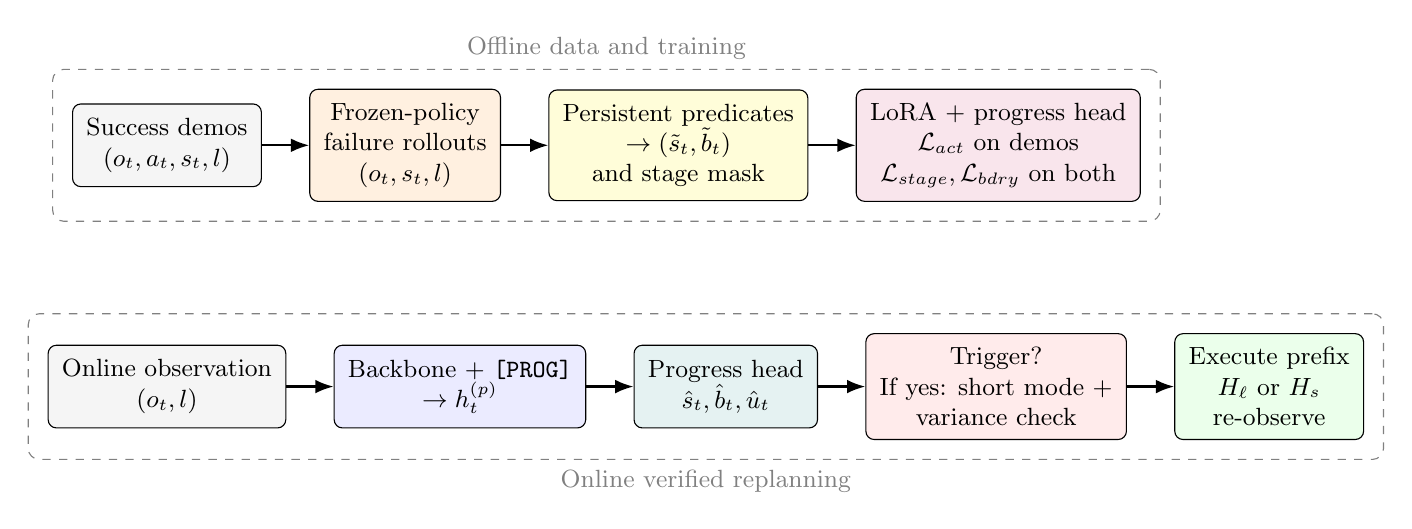
\begin{tikzpicture}[
  font=\small,
  box/.style={draw, rounded corners=3pt, inner sep=5pt, align=center,
              minimum height=1.05cm, minimum width=2.1cm},
  arrow/.style={-Latex, thick},
  dbox/.style={draw, dashed, rounded corners=4pt, inner sep=7pt, gray}
]
\node[box, fill=gray!8] (demo) at (0,0)
  {Success demos\\$(o_t,a_t,s_t,l)$};
\node[box, fill=orange!12, right=0.6cm of demo] (fail)
  {Frozen-policy\\failure rollouts\\$(o_t,s_t,l)$};
\node[box, fill=yellow!15, right=0.6cm of fail] (label)
  {Persistent predicates\\$\to (\st,\bt)$\\and stage mask};
\node[box, fill=purple!10, right=0.6cm of label] (train)
  {LoRA + progress head\\$\mathcal{L}_{act}$ on demos\\$\mathcal{L}_{stage},\mathcal{L}_{bdry}$ on both};
\draw[arrow] (demo) -- (fail);
\draw[arrow] (fail) -- (label);
\draw[arrow] (label) -- (train);
\node[box, fill=gray!8, below=2.0cm of demo] (obs)
  {Online observation\\$(o_t,l)$};
\node[box, fill=blue!8, right=0.6cm of obs] (enc)
  {Backbone + \progtok\\$\to h_t^{(p)}$};
\node[box, fill=teal!10, right=0.6cm of enc] (head)
  {Progress head\\$\hat s_t,\hat b_t,\hat u_t$};
\node[box, fill=red!8, right=0.6cm of head] (ctrl)
  {Trigger?\\If yes: short mode +\\variance check};
\node[box, fill=green!8, right=0.6cm of ctrl] (exec)
  {Execute prefix\\$\Hl$ or $\Hs$\\re-observe};
\draw[arrow] (obs) -- (enc);
\draw[arrow] (enc) -- (head);
\draw[arrow] (head) -- (ctrl);
\draw[arrow] (ctrl) -- (exec);
\node[dbox, fit=(demo)(train), label={[gray]above:Offline data and training}] {};
\node[dbox, fit=(obs)(exec), label={[gray]below:Online verified replanning}] {};
\end{tikzpicture}
\caption{Offline labeling and training above; online verified replanning below.
The controller changes when it re-observes and when it accepts a boundary
signal, but it does not inject a stage index into the action generator.}
\label{fig:overview}
\end{figure}

\subsection{State-grounded boundary labels and failure augmentation}
\label{sec:labels}

For each successful demonstration trajectory we compute
$\{T_k\}_{k=1}^{\Sstages}$ via Eq.~\eqref{eq:Tk}, then assign $\st$ and $\bt$
via Eqs.~\eqref{eq:stage_label} and~\eqref{eq:boundary_label}.
This gives the progress head supervision that is grounded in outcome-level
state, not proxy motion events such as gripper closure.

We additionally collect rollouts from the frozen base policy.
These trajectories are useful because they contain visually plausible but
unsuccessful boundary states: missed grasps, partial insertions, unstable object
contacts, or early releases.
We keep only the observation and simulator-state traces from these failures;
we do \emph{not} treat their actions as expert targets.
This avoids contaminating imitation learning with low-quality action labels.

Let
\[
  j^{\mathrm{fail}} = \min\{k : T_k = \infty\}
\]
for a failure rollout, if such a stage exists.
We keep the boundary label $\bt$ for the entire rollout, but define a stage-loss
mask
\begin{equation}
  m_t =
  \begin{cases}
    1, & \text{if no failure stage exists},\\
    \one[j^{\mathrm{fail}}>1 \ \wedge\  t \le T_{j^{\mathrm{fail}}-1}], & \text{otherwise.}
  \end{cases}
  \label{eq:mask}
\end{equation}
Thus the stage classifier is trained only up to the last reliably completed
boundary. If the first stage never completes, the stage loss is masked out on
that failure rollout. After the first failed stage begins, the trajectory may
drift arbitrarily, and a
hard stage label becomes misleading.
The boundary head still receives valuable negative examples because $\bt=0$
throughout the failed attempt.

\begin{algorithm}[t]
\caption{Predicate-based stage and boundary labeling}
\label{alg:labels}
\begin{algorithmic}[1]
\Require Trajectory $\tau=\{(o_t,a_t,s_t)\}_{t=0}^{T}$, ordered predicates
         $\{\phi_k\}_{k=1}^{\Sstages}$, persistence $\Delta$, anticipation window $w$
\Ensure Labels $\{(\st,\bt,m_t)\}_{t=0}^{T}$
\For{$k=1$ to $\Sstages$}
  \State Compute persistent completion time $T_k$ via Eq.~\eqref{eq:Tk}
\EndFor
\State $j^{\mathrm{fail}} \gets \min\{k : T_k=\infty\}$ if it exists
\For{$t=0$ to $T$}
  \State $\st \gets \min(\{k : t \le T_k\} \cup \{\Sstages\})$
  \State $\bt \gets \one[\exists k \text{ with } T_k<\infty \text{ and } T_k-w \le t \le T_k]$
  \If{$j^{\mathrm{fail}}$ does not exist}
    \State $m_t \gets 1$
  \Else
    \State $m_t \gets \one[j^{\mathrm{fail}}>1 \ \wedge\ t \le T_{j^{\mathrm{fail}}-1}]$
  \EndIf
\EndFor
\end{algorithmic}
\end{algorithm}

\subsection{Progress-aware parameter-efficient fine-tuning}
\label{sec:training}

We assume a chunked VLA with multimodal encoder $E_\theta$ and action generator
$G_\phi$.
For a current observation, the base policy produces a future action chunk of
length $L$:
\begin{equation}
  z_t = E_\theta(o_t,l), \qquad
  \mathbf{A}_t = G_\phi(z_t) \in \mathbb{R}^{L \times d_a}.
  \label{eq:basechunk}
\end{equation}
In SmolVLA-like systems this action expert is a flow-matching chunk generator~\cite{msplora}.
The crucial design choice in our method is that we do \emph{not} require the
policy to accept a stage index or a variable generation horizon.
The controller only chooses how much of a freshly generated chunk to execute.

We append a learned token embedding $\mathbf{p}\in\mathbb{R}^d$
(the \progtok\ token) to the backbone token sequence and take the final hidden
state at that position, $h_t^{(p)}\in\mathbb{R}^d$, as a compact progress
representation.
A lightweight MLP head $D_\psi$ predicts
\begin{align}
  \hat s_t &= \mathrm{softmax}(W_s h_t^{(p)} + b_s)
    \in \Delta^{\Sstages},
    \label{eq:head_stage}\\
  \hat b_t &= \sigma(W_b h_t^{(p)} + b_b) \in [0,1],
    \label{eq:head_boundary}\\
  \hat u_t &= \mathcal{H}(\hat s_t)
    = -\sum_{k=1}^{\Sstages} \hat s_t[k] \log \hat s_t[k]
    \in [0,\log \Sstages].
    \label{eq:head_entropy}
\end{align}
Here $\hat s_t$ is a stage distribution, $\hat b_t$ is the predicted probability
that the controller is close to a persistent boundary, and $\hat u_t$ is stage
entropy used as a trigger-side uncertainty proxy.

The action imitation loss is computed only on successful demonstrations.
Auxiliary progress losses are computed on both successful demonstrations and
failure rollouts.
Let $\mathcal{D}_{succ}$ be the set of successful demonstrations and
$\mathcal{D}_{fail}$ the set of failure rollouts.
Then
\begin{align}
  \mathcal{L}
  &= \sum_{\tau\in\mathcal{D}_{succ}} \mathcal{L}_{act}(\tau)
   + \lambda_s \sum_{\tau\in \mathcal{D}_{succ}\cup\mathcal{D}_{fail}}
      \sum_t m_t\, \mathrm{CE}(\hat s_t,\st) \\
  &\quad + \lambda_b \sum_{\tau\in \mathcal{D}_{succ}\cup\mathcal{D}_{fail}}
      \sum_t \mathrm{BCE}(\hat b_t,\bt).
  \label{eq:loss}
\end{align}
This preserves expert action supervision while using failure trajectories only
for the auxiliary progress task.

\subsection{Verified replanning by prefix execution}
\label{sec:inference}

The base policy always returns a chunk of fixed length $L$.
We set $L=\Hl$ and define two execution prefixes:
\begin{itemize}[leftmargin=1.5em, itemsep=0.15em]
  \item \textbf{long mode:} execute the first $\Hl$ actions of a newly generated
  chunk;
  \item \textbf{short mode:} execute only the first $\Hs$ actions, where
  $\Hs<\Hl$, then re-observe.
\end{itemize}
Long mode is efficient in smooth trajectory regions; short mode increases
replanning frequency near suspected boundaries.

\subsubsection{Level 1: coarse boundary trigger}

After each re-observation we compute $(\hat s_t,\hat b_t,\hat u_t)$.
A coarse trigger is raised when
\begin{equation}
  r_t = [\hat b_t > \delta_b]
  \ \vee\ [\hat u_t > \eta]
  \ \vee\ [t>0 \wedge \arg\max\hat s_t \neq \arg\max\hat s_{t-1}].
  \label{eq:trigger}
\end{equation}
If $r_t=0$ and the controller is not already accumulating confirmations, it
stays in long mode.
Otherwise it enters or remains in short mode.

\subsubsection{Level 2: variance-based acceptance rule}

When the controller is in short mode, it samples $\Msamples$ independent action
chunks from the policy at the current observation:
\[
  \{\mathbf{A}_t^{(i)}\}_{i=1}^{\Msamples}
  = \{G_\phi(z_t)\}_{i=1}^{\Msamples}.
\]
Let $\mathbf{P}_t^{(i)} = \mathrm{prefix}_{\Hs}(\mathbf{A}_t^{(i)})$ be the short
prefix of sample $i$, flattened into a vector of dimension $d_a\Hs$.
To reduce scale sensitivity across action dimensions, we whiten by a diagonal
covariance estimate $\Sigma$ computed from demonstration actions.
The variance score is
\begin{equation}
  V_t = \frac{1}{\Msamples}
  \sum_{i=1}^{\Msamples}
  \frac{1}{d_a\Hs}
  \left\|\mathrm{vec}(\mathbf{P}_t^{(i)}-\bar{\mathbf{P}}_t)\right\|_{\Sigma^{-1}}^2,
  \qquad
  \bar{\mathbf{P}}_t = \frac{1}{\Msamples}\sum_{i=1}^{\Msamples}\mathbf{P}_t^{(i)}.
  \label{eq:variance}
\end{equation}
High variance indicates that the policy assigns substantially different local
continuations to the same observation, which we interpret as ambiguity near an
unstable or failed boundary.
Low variance does \emph{not} prove that the state is correct, so we use it only
as one part of a conservative acceptance rule.

Let $q_t$ be the number of consecutive short-mode checks satisfying both
$r_t=1$ and $V_t\le\tau_V$.
The controller accepts a verified boundary event only after $C$ consecutive
confirmations, typically $C=2$:
\begin{equation}
  q_t =
  \begin{cases}
    q_{t-1}+1, & \text{if } r_t=1 \text{ and } V_t\le\tau_V,\\
    0, & \text{otherwise.}
  \end{cases}
  \label{eq:confirm}
\end{equation}
When $q_t=C$, the controller emits a verified boundary event and returns to
long mode.
If confirmation is not maintained, it keeps executing short prefixes and
re-observing.

A verified transition event changes the \emph{controller state}, not the action
model.
The policy is queried again from the new observation, but it is not explicitly
conditioned on a stage index.
This matches the public chunked-policy interface and avoids the inconsistency in
the earlier draft.

\begin{algorithm}[t]
\caption{\method\ inference controller}
\label{alg:inference}
\begin{algorithmic}[1]
\Require Instruction $l$, initial observation $o_0$, long prefix $\Hl$, short prefix $\Hs$,
         thresholds $(\delta_b,\eta,\tau_V)$, number of samples $\Msamples$,
         confirmation count $C$
\State $q \gets 0$
\While{episode not terminated}
  \State $z_t \gets E_\theta(o_t,l)$
  \State $(\hat s_t,\hat b_t,\hat u_t) \gets D_\psi(h_t^{(p)})$
  \State Compute trigger $r_t$ using Eq.~\eqref{eq:trigger}
  \If{$r_t=0$ \textbf{and} $q=0$}
    \State Sample one chunk $\mathbf{A}_t \sim G_\phi(z_t)$
    \State Execute $\mathrm{prefix}_{\Hl}(\mathbf{A}_t)$
  \Else
    \State Sample $\{\mathbf{A}_t^{(i)}\}_{i=1}^{\Msamples} \sim G_\phi(z_t)$
    \State Compute $V_t$ from the short prefixes via Eq.~\eqref{eq:variance}
    \If{$r_t=1$ \textbf{and} $V_t\le\tau_V$}
      \State $q \gets q+1$
    \Else
      \State $q \gets 0$
    \EndIf
    \State Reuse one sampled chunk and execute $\mathrm{prefix}_{\Hs}(\mathbf{A}_t^{(1)})$
    \If{$q=C$}
      \State Emit verified boundary event and set $q \gets 0$
    \EndIf
  \EndIf
  \State Re-observe
\EndWhile
\end{algorithmic}
\end{algorithm}

\subsection{Compute accounting}

The earlier draft understated compute by claiming that variance verification
fires at most once per boundary.
That is not generally true: the controller may stay in short mode for several
checks around the same boundary.
A more accurate accounting is therefore in terms of decision points, not stages.

Let $N_\ell$ be the number of long-mode decision points and $N_s$ the number of
short-mode decision points in an episode.
If one of the $\Msamples$ chunks generated in short mode is reused for action
execution, then the total number of policy chunk samples is
\begin{equation}
  C_{\mathrm{epi}} = N_\ell + \Msamples N_s.
  \label{eq:compute}
\end{equation}
The average executed prefix length is
\begin{equation}
  \bar H = \frac{N_\ell \Hl + N_s \Hs}{N_\ell + N_s}.
  \label{eq:avgH}
\end{equation}
Compared with a fixed long-prefix baseline, the cost increase depends on how
often the controller remains in short mode, not only on the number of ground-truth
subtasks.

\begin{figure}[t]
\centering
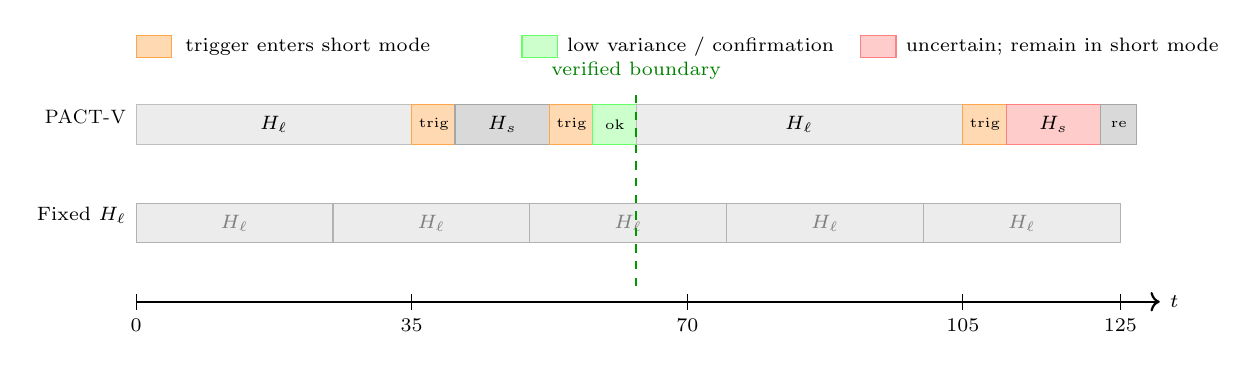
\begin{tikzpicture}[font=\small]
\draw[thick,->] (0,0) -- (13,0) node[right,font=\scriptsize]{$t$};
\foreach \x/\lab in {0/0,3.5/35,7/70,10.5/105,12.5/125}
  \draw (\x,0.1)--(\x,-0.1) node[below,font=\scriptsize]{\lab};
\node[left,font=\scriptsize] at (0,1.1) {Fixed $\Hl$};
\foreach \x in {0,2.5,5,7.5,10}
  \draw[fill=gray!15,draw=gray!60] (\x,0.75) rectangle ++(2.5,0.5);
\foreach \x/\lab in {1.25/$\Hl$,3.75/$\Hl$,6.25/$\Hl$,8.75/$\Hl$,11.25/$\Hl$}
  \node[font=\scriptsize,gray] at (\x,1.0) {\lab};
\node[left,font=\scriptsize] at (0,2.35) {\method};
\draw[fill=gray!15,draw=gray!50] (0,2.0) rectangle ++(3.5,0.5);
\node[font=\scriptsize] at (1.75,2.25) {$\Hl$};
\draw[fill=orange!30,draw=orange!70] (3.5,2.0) rectangle ++(0.55,0.5);
\node[font=\tiny] at (3.78,2.25) {trig};
\draw[fill=gray!30,draw=gray!70] (4.05,2.0) rectangle ++(1.2,0.5);
\node[font=\scriptsize] at (4.65,2.25) {$\Hs$};
\draw[fill=orange!30,draw=orange!70] (5.25,2.0) rectangle ++(0.55,0.5);
\node[font=\tiny] at (5.53,2.25) {trig};
\draw[fill=green!20,draw=green!60] (5.8,2.0) rectangle ++(0.55,0.5);
\node[font=\tiny] at (6.08,2.25) {ok};
\draw[fill=gray!15,draw=gray!50] (6.35,2.0) rectangle ++(4.15,0.5);
\node[font=\scriptsize] at (8.42,2.25) {$\Hl$};
\draw[fill=orange!30,draw=orange!70] (10.5,2.0) rectangle ++(0.55,0.5);
\node[font=\tiny] at (10.78,2.25) {trig};
\draw[fill=red!20,draw=red!50] (11.05,2.0) rectangle ++(1.2,0.5);
\node[font=\scriptsize] at (11.65,2.25) {$\Hs$};
\draw[fill=gray!30,draw=gray!70] (12.25,2.0) rectangle ++(0.45,0.5);
\node[font=\tiny] at (12.48,2.25) {re};
\draw[dashed,green!60!black,thick] (6.35,0.2)--(6.35,2.7)
  node[above,font=\scriptsize,green!50!black]{verified boundary};
\draw[fill=orange!30,draw=orange!70] (0,3.1) rectangle ++(0.45,0.28);
\node[right,font=\scriptsize] at (0.5,3.24) {trigger enters short mode};
\draw[fill=green!20,draw=green!60] (4.9,3.1) rectangle ++(0.45,0.28);
\node[right,font=\scriptsize] at (5.35,3.24) {low variance / confirmation};
\draw[fill=red!20,draw=red!50] (9.2,3.1) rectangle ++(0.45,0.28);
\node[right,font=\scriptsize] at (9.65,3.24) {uncertain; remain in short mode};
\end{tikzpicture}
\caption{The controller stays in long-prefix execution during smooth segments,
then switches to short-prefix replanning near suspected boundaries.
A boundary is accepted only after consecutive short-mode confirmations.}
\label{fig:timeline}
\end{figure}

\section{Evaluation Protocol}
\label{sec:eval}

This section describes how the method should be evaluated.
It is written as a protocol rather than a result section because the current
draft does not claim unmeasured performance gains.

\subsection{Base policy and benchmark}

We recommend evaluating \method\ on SmolVLA base, an open lightweight VLA with
chunked action generation and public PEFT support~\cite{msplora}.
For long-horizon evaluation, the primary benchmark is LIBERO-LONG, the
10-task evaluation split (\texttt{libero\_10}) of the LIBERO benchmark~\cite{libero}.
Secondary evaluation can include LIBERO-Spatial and LIBERO-Object to test whether
gains are concentrated on genuinely multi-stage tasks.

\subsection{Task decomposition and predicate release}

The method requires an ordered list of stage predicates per task.
These predicates should be released with the code and must be specified before
running evaluation.
For reproducibility, each task should provide stage names, exact predicate
definitions, the persistence parameter $\Delta$, the anticipation window $w$,
and the matching window $\omega$ used when scoring boundary recall.
This is preferable to listing guessed environment keys in the paper, because the
relevant state features can differ across tasks and simulator wrappers.

\subsection{Training and data construction}

Successful demonstrations are used for action imitation and progress
supervision.
Failure augmentation is built from rollouts of the frozen base policy on the
training tasks.
Only observation-state traces are retained for the auxiliary progress losses.
The action imitation loss remains demonstration-only.

All controller thresholds must be selected on a validation set containing both
successful demonstrations and failure rollouts.
Tuning only on successful demonstrations is insufficient because false-positive
transitions are negative events.

\subsection{Baselines}

A minimal evaluation should compare against:
\begin{itemize}[leftmargin=1.5em, itemsep=0.15em]
  \item the frozen base policy with fixed long-prefix execution,
  \item the same policy with fixed short-prefix execution,
  \item progress head without failure augmentation,
  \item progress head with failure augmentation but without variance-based
  verification, and
  \item external long-horizon baselines such as PALM or CycleVLA when a faithful
  reproduction is possible~\cite{palm,cyclevla}.
\end{itemize}
Because external baselines may require additional modules or training recipes,
any comparison should clearly separate same-backbone ablations from cross-paper
baselines.

\subsection{Metrics}

Let $\mathcal{E}$ denote the accepted boundary events emitted by the controller.
For each stage with finite persistent completion time $T_k$, we consider a
matched detection successful if some accepted boundary event falls within the
window $[T_k-\omega,\,T_k+\omega]$.
We recommend reporting the following metrics.
\begin{itemize}[leftmargin=1.5em, itemsep=0.15em]
  \item \textbf{Task success rate (SR).}
  Fraction of evaluation episodes that satisfy the environment success criterion.
  \item \textbf{False-positive transition rate (FPT).}
  \begin{equation}
    \mathrm{FPT}
    = \frac{\#\{e\in\mathcal{E}: e \text{ satisfies Eq.~\eqref{eq:fptdef}}\}}
    {\max(1,|\mathcal{E}|)}.
    \label{eq:metric_fpt}
  \end{equation}
  \item \textbf{Boundary recall (BR).}
  Fraction of ground-truth stage completions that are matched by at least one
  accepted boundary event in the tolerance window.
  \item \textbf{Blocked-trigger rate (BTR).}
  Fraction of coarse trigger activations that do not become accepted boundary
  events within the next $C$ short-mode checks.
  This measures controller conservativeness and should \emph{not} be confused
  with FPT.
  \item \textbf{Normalized chunk-sample cost.}
  Report $C_{\mathrm{epi}}$ from Eq.~\eqref{eq:compute}, normalized by the fixed
  long-prefix baseline.
\end{itemize}

\subsection{Suggested initial search ranges}

Reasonable starting ranges for the controller are:
\[
  \Hs \in \{4,5,6\}, \qquad
  \Hl \in \{16,20,24\}, \qquad
  \Msamples \in \{4,8,12\}, \qquad
  C \in \{2,3\}.
\]
Thresholds $(\delta_b,\eta,\tau_V)$ should be selected jointly on validation data,
optimizing a boundary-quality metric such as boundary F1 under a compute budget.
Because $\tau_V$ depends on action scaling and policy stochasticity, it is
expected to be the most sensitive parameter.

\section{Limitations and Expected Failure Modes}
\label{sec:limitations}

Low action variance does not guarantee that the state is correct; a model can be
confidently wrong.
Conversely, high variance may occur in genuinely multimodal but valid states.
That is why we use variance only as a conservative rejection signal and combine
it with repeated short-horizon re-observation.

The method depends on explicit task decompositions and stage predicates.
That is practical in simulation, but real-world deployment would require either
instrumented environments or learned predicate estimators.

\method\ improves boundary handling but does not backtrack, replan semantically,
or recover from large upstream failures the way a heavier external verifier might
attempt~\cite{cyclevla}.
If a task leaves the training distribution badly enough, short-mode replanning
alone may not recover it.

This is also a design choice, not a bug.
The benefit is interface simplicity and compatibility with public chunked VLA
implementations.
The downside is that \method\ cannot intentionally switch to stage-specialized
action distributions; it can only control how often the policy is queried and
when a transition is accepted.

\section{Conclusion}

We presented a corrected version of \method, a lightweight method for
boundary-aware replanning in chunked VLA policies.
The key idea is to treat long-horizon robustness as a transition-handling
problem rather than a full architecture redesign problem.
State-grounded predicate labels provide clean supervision for when boundaries are
approaching, failure rollouts teach the progress head about visually plausible
negative outcomes, and variance-based short-mode replanning offers a practical
way to reject premature transitions without external modules.

Equally important, this draft makes explicit what the method does \emph{not}
claim.
It does not prove correctness, it does not change the base policy into a
subtask-conditioned controller, and it does not report gains that have not yet
been measured.
Instead, it offers an internally consistent algorithm and a reproducible
experimental protocol for testing whether verified boundary handling improves
long-horizon success in lightweight VLAs.

\begin{thebibliography}{99}

% ---- Foundational VLA models ----

\bibitem{openvla}
Moo Jin Kim, Karl Pertsch, Siddharth Karamcheti, Ted Xiao, Ashwin Balakrishna,
Suraj Nair, Rafael Rafailov, Ethan Foster, Grace Lam, Pannag Sanketi, and others.
\newblock OpenVLA: An Open-Source Vision-Language-Action Model.
\newblock \emph{arXiv preprint arXiv:2406.09246}, 2024.

\bibitem{rt2}
Anthony Brohan, Noah Brown, Justice Carbajal, Yevgen Chebotar, Joseph Dabis,
Chelsea Finn, Keerthana Gopalakrishnan, Karol Hausman, Alex Herzog,
Jasmine Hsu, and others.
\newblock RT-2: Vision-Language-Action Models Transfer Web Knowledge
to Robotic Control.
\newblock \emph{arXiv preprint arXiv:2307.15818}, 2023.

\bibitem{msplora}
Mustafa Shukor, Dana Aubakirova, Francesco Capuano, Pepijn Kooijmans,
Steven Morad, and others.
\newblock SmolVLA: A Vision-Language-Action Model for Affordable and
Efficient Robotics.
\newblock \emph{arXiv preprint arXiv:2506.01844}, 2025.

% ---- Benchmark ----

\bibitem{libero}
Bo Liu, Yifeng Zhu, Chongkai Gao, Yihao Feng, Qiang Liu,
Yuke Zhu, and Peter Stone.
\newblock LIBERO: Benchmarking Knowledge Transfer for Lifelong Robot Learning.
\newblock \emph{arXiv preprint arXiv:2306.03310}, 2023.

% ---- Long-horizon: progress, self-correction, memory ----

\bibitem{palm}
Yuanzhe Liu, Jingyuan Zhu, Yuchen Mo, Gen Li, Qianning Guo,
Xiaoqian Liu, Fengming Li, Yimin Zhang, Zhenyu Huang, Hao Tang,
Bin Liang, and others.
\newblock PALM: Progress-Aware Policy Learning via Affordance Reasoning
for Long-Horizon Robotic Manipulation.
\newblock \emph{arXiv preprint arXiv:2601.07060}, 2026.

\bibitem{cyclevla}
Chenyang Ma, Guangyu Yang, Kai Lu, Shitong Xu, Bill Byrne,
Niki Trigoni, and Andrew Markham.
\newblock CycleVLA: Proactive Self-Correcting Vision-Language-Action Models
via Subtask Backtracking and Minimum Bayes Risk Decoding.
\newblock \emph{arXiv preprint arXiv:2601.02295}, 2026.

\bibitem{robocerebra}
Han and others.
\newblock RoboCerebra: A Large-Scale Benchmark for Long-Horizon Robotic
Manipulation Evaluation.
\newblock \emph{arXiv preprint arXiv:2506.06677}, 2025.

\bibitem{vlasct}
Wentao Zhang, Aolan Sun, and others.
\newblock From Knowing to Doing Precisely: A General Self-Correction and
Termination Framework for VLA Models.
\newblock \emph{arXiv preprint arXiv:2602.01811}, 2026.

\bibitem{subgoaltransition}
Anonymous.
\newblock Enabling Long(er) Horizon Imitation for Manipulation Tasks
by Modeling Subgoal Transitions.
\newblock In \emph{OpenReview}, 2025.
\newblock \url{https://openreview.net/forum?id=fBRqCMqVyS}

% ---- Phase-aware and RL-based progress ----

\bibitem{longhorizonvla}
Yiguo Fan, Peng Ding, Siyuan Bai, Xinwang Tong, Yuke Zhu,
Hang Lu, Fei Dai, Wei Zhao, Yao Liu, Shu Huang, and others.
\newblock Long-VLA: Unleashing Long-Horizon Capability of Vision Language
Action Model for Robot Manipulation.
\newblock In \emph{Conference on Robot Learning (CoRL)}, 2025.
\newblock \emph{arXiv preprint arXiv:2508.19958}.

\bibitem{grrl}
Go and others.
\newblock GR-RL: Going Dexterous and Precise for Long-Horizon Robotic
Manipulation.
\newblock \emph{arXiv preprint arXiv:2512.01801}, 2025.

% ---- Memory-augmented approaches ----

\bibitem{lola}
Zixuan Chen, Jianlong Fu, and others.
\newblock LoLA: Long Horizon Latent Action Learning for General
Robot Manipulation.
\newblock \emph{arXiv preprint arXiv:2512.20166}, 2025.

\bibitem{slotssm}
Huy Le and others.
\newblock Rethinking Progression of Memory State in Robotic Manipulation:
An Object-Centric Perspective.
\newblock \emph{arXiv preprint arXiv:2511.11478}, 2025.

% ---- Adaptive action chunking ----

\bibitem{reactivedp}
Lili Chen and others.
\newblock Reactive Diffusion Policy: Slow-Fast Visual-Tactile Policy Learning
for Contact-Rich Manipulation.
\newblock \emph{arXiv preprint}, 2024.

\bibitem{sgac}
Che and others.
\newblock SGAC: Similarity-Guided Adaptive Chunking for Diffusion Policies.
\newblock \emph{arXiv preprint}, 2024.

\bibitem{radp}
Chen and others.
\newblock RA-DP: Replanning-Augmented Diffusion Policy for Adaptive
Robot Manipulation.
\newblock \emph{arXiv preprint}, 2024.

% ---- Imitation learning theory ----

\bibitem{ross2011dagger}
Stephane Ross, Geoffrey Gordon, and Drew Bagnell.
\newblock A Reduction of Imitation Learning and Structured Prediction to
No-Regret Online Learning.
\newblock In \emph{Proceedings of the Fourteenth International Conference on
Artificial Intelligence and Statistics (AISTATS)}, pages 627--635, 2011.

\end{thebibliography}

\appendix

\section{Predicate specification template}
\label{app:predicates}

To avoid hard-coding unverifiable environment keys in the manuscript, each task
should release a separate predicate sheet with the following fields.

\begin{table}[h]
\centering
\caption{Per-task predicate specification template.}
\label{tab:predicate_template}
\begin{tabular}{p{2.1cm}p{2.0cm}p{6.4cm}}
\toprule
Field & Symbol & Description \\
\midrule
Stage name & $g_k$ & Human-readable subtask name (e.g., reach, grasp, align, place) \\
Predicate & $\phi_k$ & Exact simulator-state condition defining persistent completion \\
Persistence & $\Delta$ & Number of consecutive satisfied timesteps required for Eq.~\eqref{eq:Tk} \\
Boundary window & $w$ & Number of pre-completion steps labeled as boundary-imminent \\
Eval window & $\omega$ & Matching tolerance for scoring boundary recall \\
Notes & --- & Task-specific caveats such as contact hysteresis or multi-object dependencies \\
\bottomrule
\end{tabular}
\end{table}

\section{Reporting checklist}
\label{app:reporting}

A complete experimental report for \method\ should include:
\begin{enumerate}[leftmargin=1.5em, itemsep=0.15em]
  \item task-level stage decompositions and predicate definitions,
  \item the number of successful demonstrations and failure rollouts used for each suite,
  \item whether LoRA was applied to the encoder only or to the shared policy blocks,
  \item the validation procedure used to tune $(\delta_b,\eta,\tau_V,\Hs,\Hl,\Msamples,C)$,
  \item SR, FPT, BR, BTR, and normalized compute with confidence intervals across seeds,
  \item ablations removing failure augmentation and variance verification, and
  \item qualitative examples of both true and false accepted boundary events.
\end{enumerate}

\end{document}